% Results v2 (19 Nov 2026). Every number comes from docs/results_ledger.md or paper/tables/tab_main.tex (generated and
% cross-checked by scripts/make_results_table.py). The old results.tex is kept for reference. Do not retype numbers from memory.

\section{Results}
\label{sec:results}

\begin{table*}[t]
\centering
\caption{Pooled RMSE ($^\circ$C) on the deep set. Against GLORYS: mean of the per-depth MSE over 15 depths. Against Argo: all matched profile-depth values at 14 levels (5--1000~m), equally weighted ($48522$, $139583$ and $6895$ values in Tests~A, B and C; Test~C has 507 profiles). The two pooling rules are not comparable in magnitude. Corrected: one additive constant per depth, fitted on validation-window Argo only. Argo is assimilated by GLORYS and is not independent of it. In the corrected columns the GLORYS12 row is GLORYS12 with its own per-depth constants applied. Best learned model in bold per column (GLORYS12 and climatology excluded).}
\label{tab:main}
\begin{tabular}{@{}lccccccccc@{}}
\hline
 & \multicolumn{3}{c}{vs GLORYS} & \multicolumn{3}{c}{vs Argo, raw} & \multicolumn{3}{c}{vs Argo, corrected} \\
\cline{2-4}\cline{5-7}\cline{8-10}
Model & A & B & C & A & B & C & A & B & C \\
\hline
Climatology & 0.969 & 1.068 & 0.906 & 1.009 & 1.106 & 0.817 & -- & -- & -- \\
Linear (SLA+SST) & 0.683 & 0.746 & 0.670 & 0.861 & 0.932 & 0.831 & 0.782 & 0.869 & 0.697 \\
XGBoost & 0.682 & 0.741 & 0.639 & 0.855 & 0.920 & 0.777 & 0.779 & 0.863 & 0.668 \\
Single U-Net & 0.690 & 0.745 & 0.642 & 0.848 & 0.917 & 0.779 & 0.776 & 0.864 & 0.668 \\
U-Net ensemble & \textbf{0.671} & \textbf{0.728} & \textbf{0.637} & 0.834 & 0.909 & 0.773 & \textbf{0.757} & \textbf{0.843} & \textbf{0.661} \\
Ensemble, demeaned SLA & 0.743 & 0.810 & 0.705 & \textbf{0.754} & \textbf{0.848} & \textbf{0.649} & 0.791 & 0.879 & 0.698 \\
\hline
GLORYS12 & -- & -- & -- & 0.677 & 0.783 & 0.711 & 0.641 & 0.735 & 0.668 \\
\hline
\end{tabular}
\end{table*}


\subsection{Agreement with GLORYS}
Against GLORYS, the frozen ensemble has a pooled deep-set RMSE of 0.671, 0.728 and 0.637$^\circ$C on Tests~A, B and C (Table~\ref{tab:main}), against 0.683, 0.746 and 0.670$^\circ$C for the per-cell linear regression and 0.969, 1.068 and 0.906$^\circ$C for the seasonal climatology. Its gain over the linear regression is $-1.8\%$ (95\% interval $[-2.9,-0.7]$), $-2.4\%$ ($[-3.2,-1.6]$) and $-4.9\%$ ($[-7.2,-3.0]$). The pre-registered prediction for the prospective Test~C, a gain of a few percent at most, held in direction, but the gain is about twice that of Tests~A and B. Over XGBoost the gain is $-1.6\%$ ($[-2.9,-0.5]$) and $-1.7\%$ ($[-2.6,-0.9]$) on Tests~A and B, and a tie on Test~C ($-0.3\%$, $[-1.7,+1.8]$).

\begin{figure*}[t]
\centering
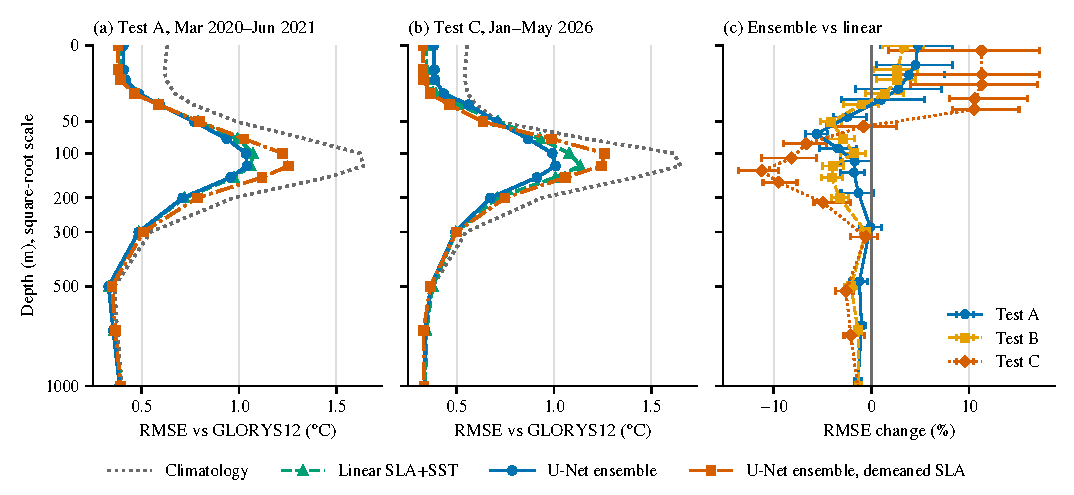
\includegraphics[width=\textwidth]{figures/fig_rmse_by_depth_v2.pdf}
\caption{(a)~RMSE against GLORYS12 by depth on the deep set for Test~A and (b)~for Test~C. (c)~RMSE change of the U-Net ensemble relative to the linear regression with 95\% block-bootstrap intervals for Tests~A, B and C (negative is better; Test~B is shown only here); points are offset vertically for legibility. The depth axis is a square-root scale.}
\label{fig:depth}
\end{figure*}

The gain is concentrated in the thermocline (Fig.~\ref{fig:depth}): at 50--200~m it is $-2.8\%$, $-3.2\%$ and $-7.9\%$ ($[-9.8,-6.2]$ on Test~C). Near the surface the ensemble is worse than the linear regression, by $2.7$--$4.8\%$ at 0--10~m on Tests~A and B (at most $0.02^\circ$C) and by $10.9\%$ ($[+6.2,+15.8]$) at 0--30~m on Test~C. Below 300~m the gains are at most about $0.01^\circ$C ($-1.5\%$, $[-2.3,-0.6]$, on Test~C), and we do not count them as skill. The demeaned ensemble, pre-registered as co-primary, is $10.7$--$11.2\%$ worse than the frozen ensemble against GLORYS in all three periods.

\subsection{Agreement with Argo profiles}
Against Argo, GLORYS itself has an RMSE of 0.677, 0.783 and 0.711$^\circ$C, and the frozen ensemble 0.834, 0.909 and 0.773$^\circ$C (Table~\ref{tab:main}). The ensemble is closer to Argo than the linear regression by $3.1\%$ ($[-5.3,-1.3]$), $2.5\%$ ($[-3.8,-1.3]$) and $7.0\%$ ($[-10.9,-3.5]$), but only at 75--200~m ($-5.5\%$, $-5.5\%$, $-10.3\%$); at 5--50~m it is worse ($+3.8\%$, $+2.7\%$, $+8.8\%$). The ranking of the two ensembles reverses with the reference: the demeaned ensemble is the closest learned model to Argo, by $9.7\%$ ($[-12.8,-7.7]$), $6.7\%$ ($[-8.5,-4.9]$) and $16.1\%$ ($[-20.1,-14.4]$) relative to the frozen ensemble. On Test~C its RMSE (0.649$^\circ$C) is below that of GLORYS, which we do not read as better than GLORYS: the period covers one season, with 507 profiles, and the reason below applies.

The reason is bias, not pattern. In the thermocline (75--200~m) the models inherit the warm bias of GLORYS relative to Argo (on Test~C: GLORYS $+0.403$, frozen $+0.607$, linear $+0.771^\circ$C). After removing each year's mean bias (2018--2025), the demeaned and frozen ensembles have the same RMSE (1.024 and 1.026$^\circ$C), so the demeaned advantage is a bias reduction; its yearly bias changes sign.

\subsection{A bias correction against Argo}
We therefore tested the simplest remedy. For each depth we subtract one constant, the mean model-minus-Argo difference on the validation-window Argo profiles (up to $0.51^\circ$C at 100--125~m), from every prediction. This analysis was specified in a pre-registration after the test periods had been scored (pre-specified, not blind), and uses no test data to fit anything. Its success rule was met: the corrected frozen ensemble is closer to Argo than the uncorrected one by $9.3\%$ ($[-11.8,-7.8]$), $7.2\%$ ($[-8.4,-6.2]$) and $14.6\%$ ($[-16.3,-14.1]$) on Tests~A, B and C, at the cost of agreement with GLORYS (0.671 to 0.716, 0.728 to 0.785 and 0.637 to 0.649$^\circ$C).

One pre-registered prediction failed: P2 expected the correction to help less than the demeaned ensemble does. Against the uncorrected demeaned ensemble, the corrected frozen ensemble differs by $+0.4\%$ ($[-0.5,+1.5]$), $-0.6\%$ ($[-2.2,+0.8]$) and $+1.9\%$ ($[+0.1,+4.9]$): one constant per depth recovers essentially the whole demeaned advantage against Argo. The correction is standard practice and is not offered as a method.

As an exploratory check, chosen after seeing these results, we applied the same rule to every estimate. The correction improves the linear regression by $9.1\%$, $6.8\%$ and $16.1\%$ and GLORYS by $5.3\%$, $6.1\%$ and $6.0\%$. The corrected ensemble stays ahead of the corrected linear regression ($-3.2\%$, $-2.9\%$, $-5.2\%$; at 75--200~m $-4.7\%$, $-5.5\%$, $-7.3\%$) and, by less, of corrected XGBoost ($-2.9\%$, $-2.2\%$, and $-1.1\%$ with interval $[-3.0,+0.5]$ on Test~C) and of the corrected single U-Net ($-2.4\%$, $-2.4\%$, $-1.1\%$). The near-surface deficit disappears, so it was bias: at 5--50~m the corrected ensemble ties the corrected linear regression in all three periods. Corrected GLORYS remains closer to Argo than the corrected ensemble on Tests~A and B ($+18.0\%$ and $+14.7\%$), with a tie on Test~C ($-1.1\%$, $[-6.7,+6.7]$).

\subsection{Further observations}
Exploratory and not pre-registered: XGBoost, which receives the day of year, was better than the ensemble at 30--50~m in January--May of six of seven years (point estimates; $+19.2\%$ at 30~m and $+22.1\%$ at 50~m in 2026, with a reversal in 2024); we do not claim a cause. Against GLORYS, among the Arabian Sea, Bay of Bengal and Andaman Sea, only the Bay of Bengal shows a gain over the linear regression with intervals excluding zero in both Test~A and Test~B ($-5.6\%$, $-3.8\%$); the validation-window advantage in the Andaman Sea ($-12.5\%$) did not replicate. Integrated Gradients on 19 validation days show reliance on SST near the surface (share 0.63 at 0~m) and on sea level at depth (0.72 at 50~m, 0.84 at 150~m); this is reliance, not correctness.
